\documentclass[conference]{IEEEtran}
\IEEEoverridecommandlockouts{}

\usepackage{cite}
\usepackage{amsmath,amssymb,amsfonts}
\usepackage{algorithmic}
\usepackage{graphicx}
\usepackage{textcomp}
\usepackage{xcolor}
\usepackage{float}
\def\BibTeX{{\rm B\kern-.05em{\sc i\kern-.025em b}\kern-.08em
    T\kern-.1667em\lower.7ex\hbox{E}\kern-.125emX}}
\begin{document}

\title{Análisis de caso | Taller II \\}

\author{
	\IEEEauthorblockN{1\textsuperscript{st} Mauro Alonso Gonzalez Figueroa}
	\IEEEauthorblockA{\textit{Universidad Tecnologica de Bolivar} \\
		\textit{UTB}\\
		Cartagena, Colombia \\
		maugonzalez@utb.edu.co \\
		T00067622}

	\and

	\IEEEauthorblockN{2\textsuperscript{st} María Valentina Serna González}
	\IEEEauthorblockA{\textit{Universidad Tecnologica de Bolivar} \\
		\textit{UTB}\\
		Cartagena, Colombia \\
		maserna@utb.edu.co \\
		T00067756}
}

\maketitle

\bibliographystyle{IEEEtran}

\begin{abstract}
	This study presents a statistical analysis of the given case,
	examining the relationship between sales and advertising expenditures. Data
	on \textit{Sales} and \textit{Advertising} were collected for a sample of 60
	companies and analyzed using Excel and Statgraphics.

	The results of the study showed a positive and moderate correlation
	between sales and advertising, with a determination coefficient \textit{($R^2$)} of
	$0,6343$. The covariance was $5,3493$, and Pearson's test indicated a
	statistical significance of $0,7964$.

	Based on these results, we conclude that sales and advertising expenditures
	are positively associated. This study provides empirical evidence on
	the connection between advertising and sales in this case.
\end{abstract}

\begin{IEEEkeywords}
	Determination coefficient, Covariance, Pearson Test, Statistical Analysis
\end{IEEEkeywords}

\section{Introducción}

El presente estudio tiene como objetivo analizar la relación entre dos
variables: Ventas y Publicidad, utilizando un conjunto de datos de 60 empresas.
Se aplicarán métodos estadísticos para determinar si existe una correlación
significativa entre las variables y comprender la naturaleza de la relación.

El análisis se basa en los siguientes métodos:

\begin{itemize}
	\item Coeficiente de determinación: Medirá la fuerza y la dirección de la
	      relación lineal entre las
	      variables~\cite{coeficiente_determinacion}.

	\item Covarianza: Indicará la variación conjunta de las
	      variables~\cite{covarianza}.

	\item Test de Pearson: Evaluará la significancia estadística de
	      la correlación~\cite{test_pearson}.
\end{itemize}

Los resultados de este estudio proporcionarán información valiosa sobre la
relación entre las variables en el contexto específico del conjunto de datos.
Se espera que la investigación contribuya a una mejor comprensión de cómo la
publicidad puede influir en las ventas, con aplicaciones potenciales para la
toma de decisiones estratégicas en el ámbito empresarial.

\section{Formulas utilizadas}

\begin{itemize}
	\item Covarianza:

	      \begin{equation}
		      C_{xy} = \frac{\Sigma xy - N \overline{x}  \overline{y} }{N - 1}
	      \end{equation}

	\item Test de Pearson:

	      \begin{equation}
		      r_{xy} = \frac{C_{xy}}{S_{x} S_{y}}
	      \end{equation}

	      \begin{equation}
		      S_{x}^{2} = \frac{\Sigma x^{2} - N {(\overline{x})}^{2}}{N - 1}
	      \end{equation}

	      \begin{equation}
		      S_{y}^{2} = \frac{\Sigma y^{2} - N {(\overline{y})}^{2}}{N - 1}
	      \end{equation}

	      \begin{equation}
		      \therefore r_{xy} = \frac{N \Sigma xy - (\Sigma x) (\Sigma y)}{\sqrt{[N \Sigma (x^{2}) - {(\Sigma x)}^{2}] [N \Sigma (y^{2}) - {(\Sigma y)}^{2}]}}
		      \label{eq:pearson_coefficient}
	      \end{equation}


	\item Coeficiente de determinación:

	      \begin{equation}
		      R^{2} = r_{xy}^{2}
		      \label{eq:r2}
	      \end{equation}


	\item Recta modelo:

	      \begin{equation}
		      y = mx + b
	      \end{equation}


	      \begin{equation}
		      m = \frac{S_{xy}}{S_{x}} = \frac{N \Sigma xy - (\Sigma x)(\Sigma y)}{N \Sigma (x^{2}) - {(\Sigma x)}^{2}}
		      \label{eq:m}
	      \end{equation}

	      \begin{equation}
		      b = \overline{y} - \textit{m} \overline{x} = \frac{\Sigma y}{N} - \textit{m} \frac{\Sigma x}{N}
		      \label{eq:b}
	      \end{equation}
\end{itemize}

\section{Preguntas a responder}

\begin{enumerate}
	\item El diagrama de dispersión o puntos para las dos variables, y observar algún patrón entre
	      ellas, como se están correlacionando, por ejemplo, si puede considerarse lineal (Copiar
	      como imagen de la herramienta de cómputo Statgraphics o Excel).

	\item El coeficiente de correlación, tratando de obtener un coeficiente numérico que nos
	      indique como se están correlacionando las dos variables (cálculos en tabla construida
	      con Excel para aplicar en fórmula).

	\item El modelo de regresión lineal que mejor se ajuste a los datos (ecuación de la recta
	      estimada y la imagen de la herramienta de cómputo con la recta obtenida), si las
	      variables están correlacionadas linealmente (cálculos manuales de las constantes,
	      aplicar fórmula).

	\item El coeficiente de determinación o bondad de ajuste, R2, de plantear un modelo de
	      regresión lineal simple ¿Se considera un buen modelo? (calcular manual, aplicar
	      fórmula).
\end{enumerate}

\section{Desarrollo}

\begin{enumerate}
	\item \hfill{}
	      \begin{figure}[H]
		      \begin{center}
			      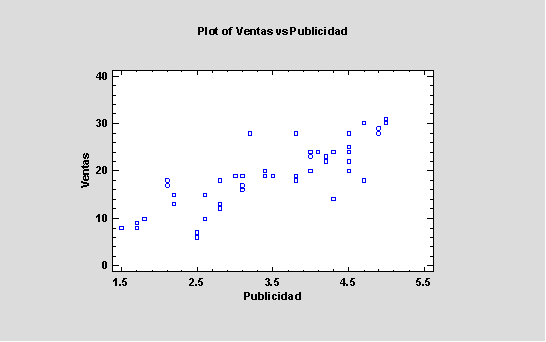
\includegraphics[width=\linewidth]{./Images/DiagramaDispersion.png}
		      \end{center}
	      \end{figure}

	      \begin{itemize}
		      \item El diagrama de dispersión proporciona evidencia de una relación
		            positiva y lineal entre las variables ``Ventas'' y ``Publicidad''.

		      \item La mayoría de los puntos se ajustan a la tendencia general, lo que
		            indica una fuerte correlación entre las variables.

		      \item Hay algunos puntos atípicos que pueden ser causados por errores en
		            la medición o por factores externos.
	      \end{itemize}

	\item Para términos del análisis, se tomo como variable
	      independiente \textit{(x)} a los valores de ``Publicidad'', mientras
	      que como variable dependiente \textit{(y)}, las ``Ventas''.

	      \begin{itemize}
		      \item $\Sigma x = 207,70$
		      \item $\Sigma y = 1148,00$
		      \item $\Sigma xy = 4289,60$
		      \item $\Sigma (x^{2}) = 778,05$
		      \item $\Sigma (x^{2}) = 24624,00$
		      \item $\overline{x} = 3,46$
		      \item $\overline{y} = 19,13$
	      \end{itemize}

	      Por lo tanto, utilizando la formula~(\ref{eq:pearson_coefficient}),
	      se obtiene un valor de $0,796414177$. Resultando en una correlación
	      lineal moderada positiva.

	\item Aplicando las formulas~(\ref{eq:m}) y~(\ref{eq:b}), obtenemos los
	      valores,

	      \begin{itemize}
		      \item $m = 5,343665255$
		      \item $b = 0,635345443$
	      \end{itemize}

	      Resultando en la recta,

	      \begin{equation*}
		      y = 5,343665255 x + 0,635345443
	      \end{equation*}

	      \begin{figure}[H]
		      \begin{center}
			      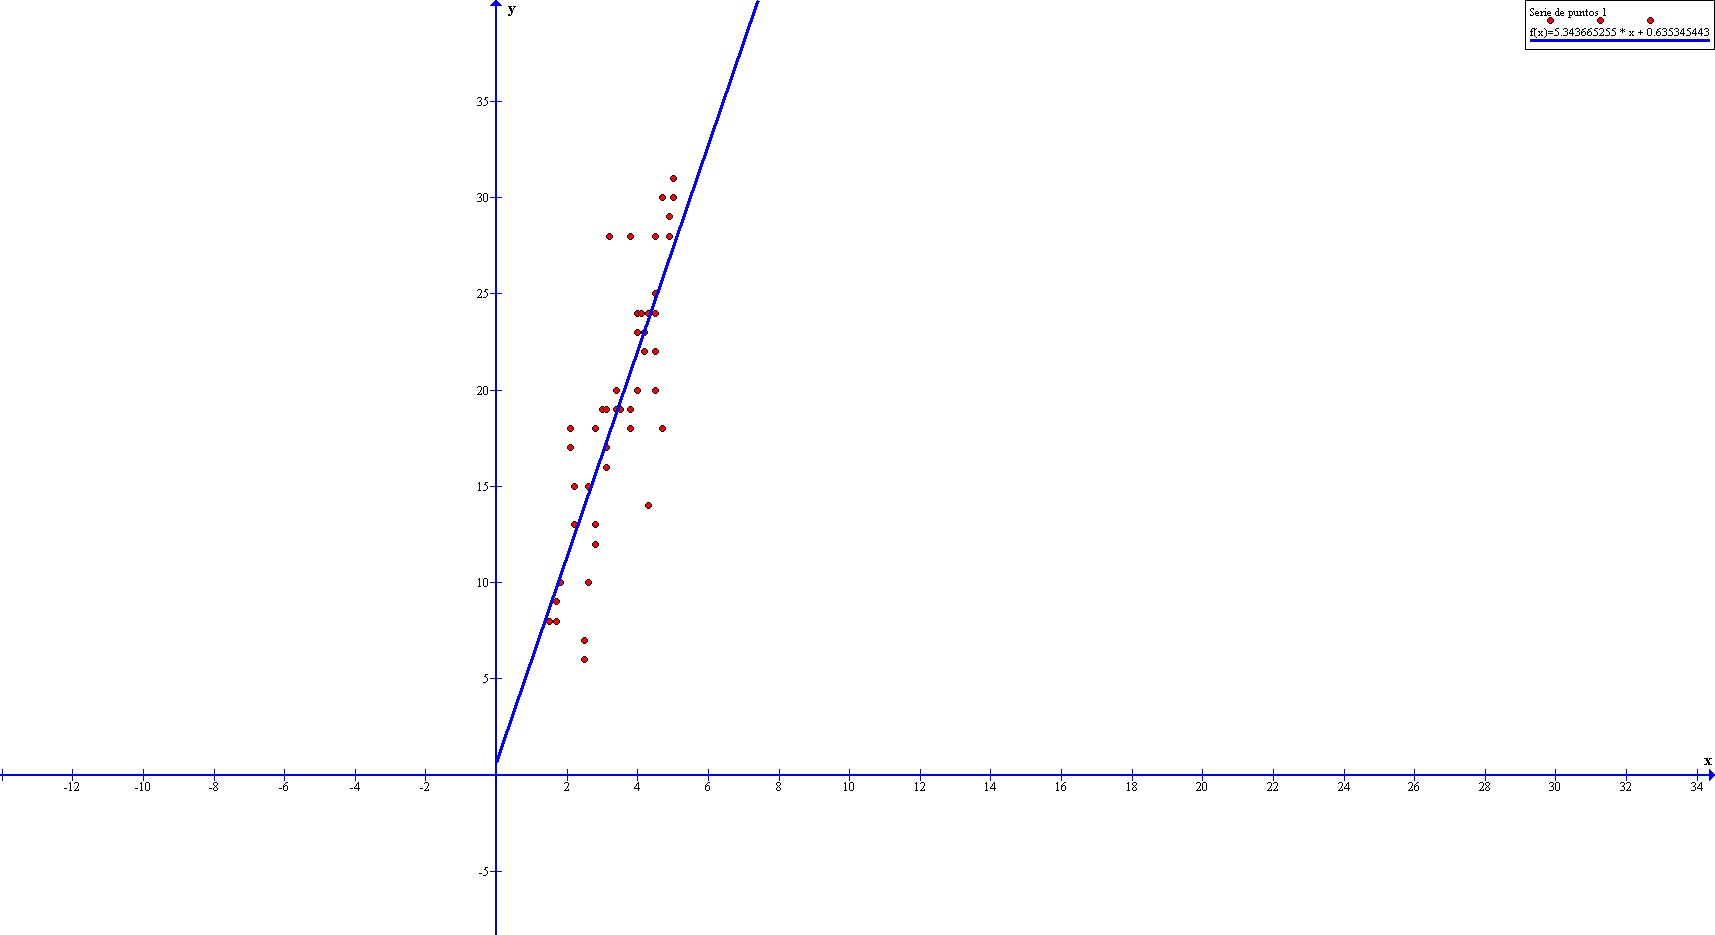
\includegraphics[width=\linewidth]{./Images/Recta.jpg}
		      \end{center}
	      \end{figure}

	\item Con el valor obtenido del test de Pearson, aplicando la
	      formula~(\ref{eq:r2}), se obtiene

	      \begin{equation*}
		      R^2 = 0,634275541 \approx 63\%
	      \end{equation*}
	      \
	      Lo cual nos dice que los datos tienen un ajuste muy bueno.

\end{enumerate}

\bibliography{./Bibliography/bibliography.bib}

\end{document}
